
We monitored the accuracy of our embeddings over the course of training our CNN. The validation set is a dataset of 1000 triplets such that 100 triplets are created from each of the 10 validation videos. After the end of training, 736/1000 samples fulfilled the triplet constraint. 930/1000 fulfilled the contrained without the added margin. I.e. $\norm{x_a - x_p} < \norm{x_a - x_n}$.

For comparison after 10 epochs of training the values were 467/1000 with margin and 894/1000 without the margin.

{
    \centering
    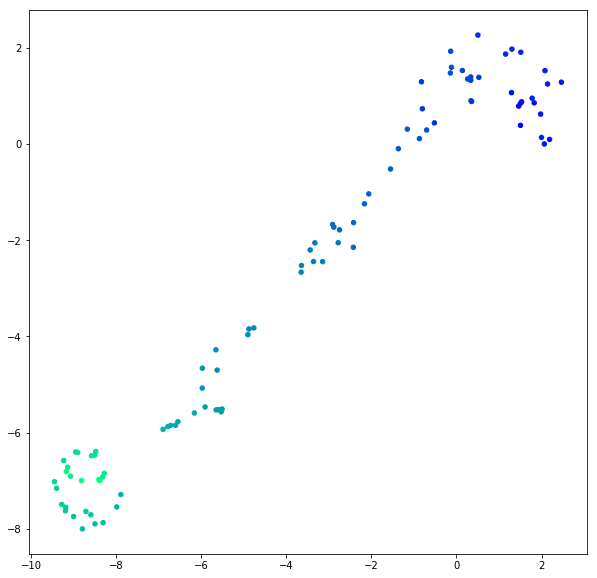
\includegraphics[width=8cm]{t-sne-trajectory.png}
    \captionof{figure}{A t-SNE plot of a validation trajectory. Perplexity 30, learning rate 200 and 1000 iterations. The color goes from blue to cyan as a function of the frame indices.}
    \label{t-sne}
    \vspace{0.25cm}
}

The t-SNE plot in figure \ref{t-sne} of a validation trajectory suggests that the network has learned a meaningful and well-behaved embedding of the video frames. Embeddings of frames that are close to each other in the video are close to each other in the dimensionality reduced regime.

{
    \centering
    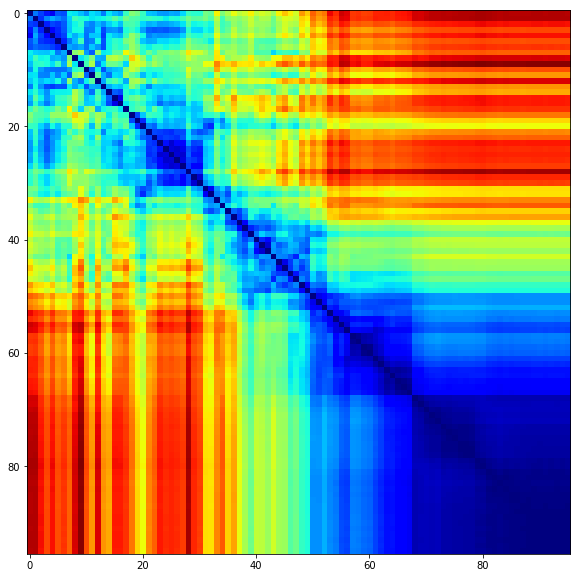
\includegraphics[width=8cm]{dima.png}
    \captionof{figure}{Visualization of the $L_2$ distance matrix of the same validation video as in figure \ref{t-sne}. Blue means close and red is far away.}
    \label{dima}
    \vspace{0.25cm}
}

{
    \centering
    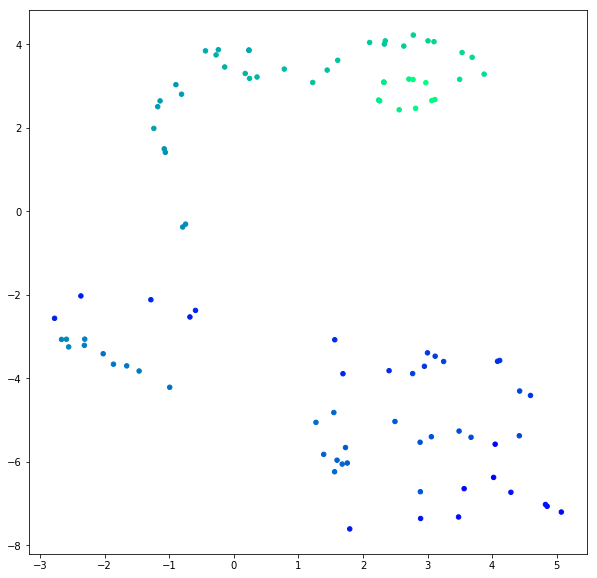
\includegraphics[width=8cm]{early_trajectory.png}
    \captionof{figure}{For comparison, a visualization of a trajectory after 50 epochs of training. Visualized using the same t-SNE parameters and the same video as figure \ref{t-sne}.}
    \label{early-t-sne}
    \vspace{0.25cm}
}
{
    \centering
    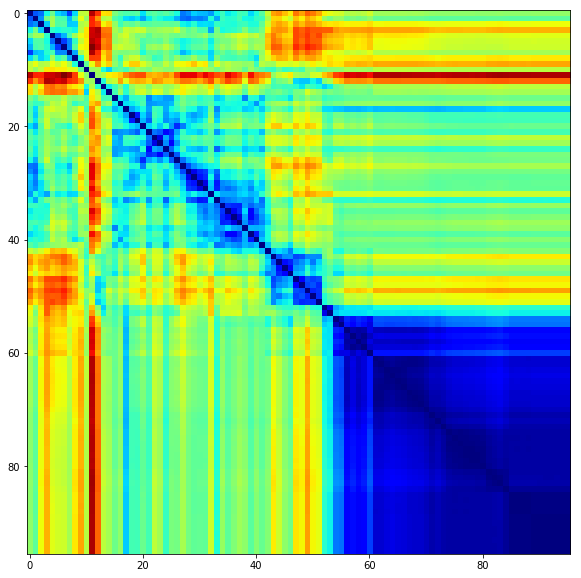
\includegraphics[width=8cm]{early-dima.png}
    \captionof{figure}{Distance matrix for the same network as in figure \ref{early-t-sne}.}
    \label{early-dima}
    \vspace{0.25cm}
}

Each row and column in the distance matrix shown in figure \ref{dima} corresponds to a frame of the video. The value is the euclidean distance between the embedding of the frame. I.e. the diagonal is 0 and the matrix is symmetric. This visualization seems to confirm that subsequent frames are close to each other in the embedding space.

Comparing figure \ref{t-sne} to figure \ref{early-t-sne} and figure \ref{dima} to figure \ref{early-dima} we can see that early on in training the network has not yet learned a meaningful embedding of the entire joint space of the robot.

First we studied performance of the PPO algorithm to generate trajectories in a simplified enviroment where a task is to move the robotic arm into a randomly sampled goal position. $L_2$ norm distance of a goal position and an robot arm position at a time step is used as a reward. The experiment indicates that the complexity of the problem is high. Figure \ref{trajectory_learning} shows learning results of the experiment. The PPO algorithm learns to generate better trajectories. However as the reward at the end of iterations show the agent accomplish to build correct trajectories for only portion of the sampled goal positions.        

{
    \centering
    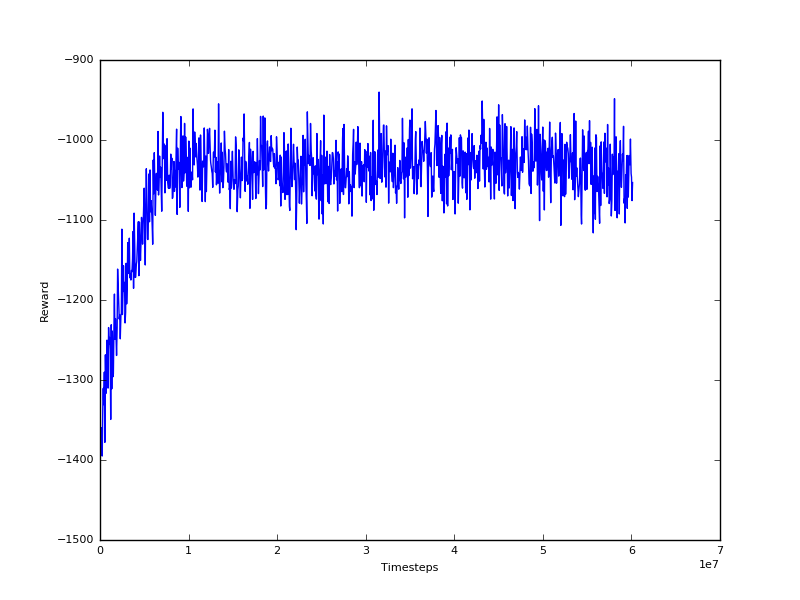
\includegraphics[width=10cm]{modified_model_1.png}
    \captionof{figure}{Learning results for moving the robot arm to a goal position}
    \label{trajectory_learning}
    \vspace{0.25cm}
}

As moving the robot arm to a randomly sampled position proved to be challenging, no remarkable achievements were expected for the imitation learning task. Hence, we experimented the imitation problem with one example video. Figure \ref{imitation} shows the achieved learning. The PPO algorithm produces trajectories that have similar features as the example video. For example, the ending pose is close to the example pose especially if we take into account that viewing angles differ. However, in the middle of the movement the position clearly differs from the example.

{
    \centering
    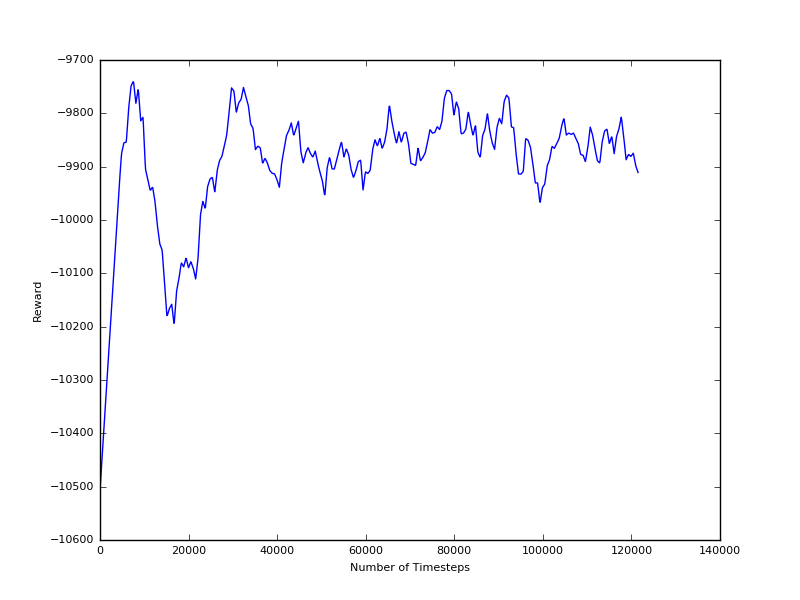
\includegraphics[width=10cm]{imitation_1.png}
    \captionof{figure}{Learning performance of the imitation}
    \label{imitation}
    \vspace{0.25cm}
}